\subsection{Attack 1, the Format String Vulnerability}

The {\tt printf, fprintf, sprintf}, etc functions in the standard C IO library are all vulnerable to format string based
attacks, which exploit the manner in which C handles calls to the class of functions they belong to: \textbf{variadic
functions}\cite{vfunc}. When a function is called in the C programming language,\cite{call_conv} the exact actions are
dependent on the specific processor architecture, compiler and operating system. In the case of the lab machines, the
situation is similar to that depicted in figure \ref{fig_stack}.

\begin{figure}[ht] \centering 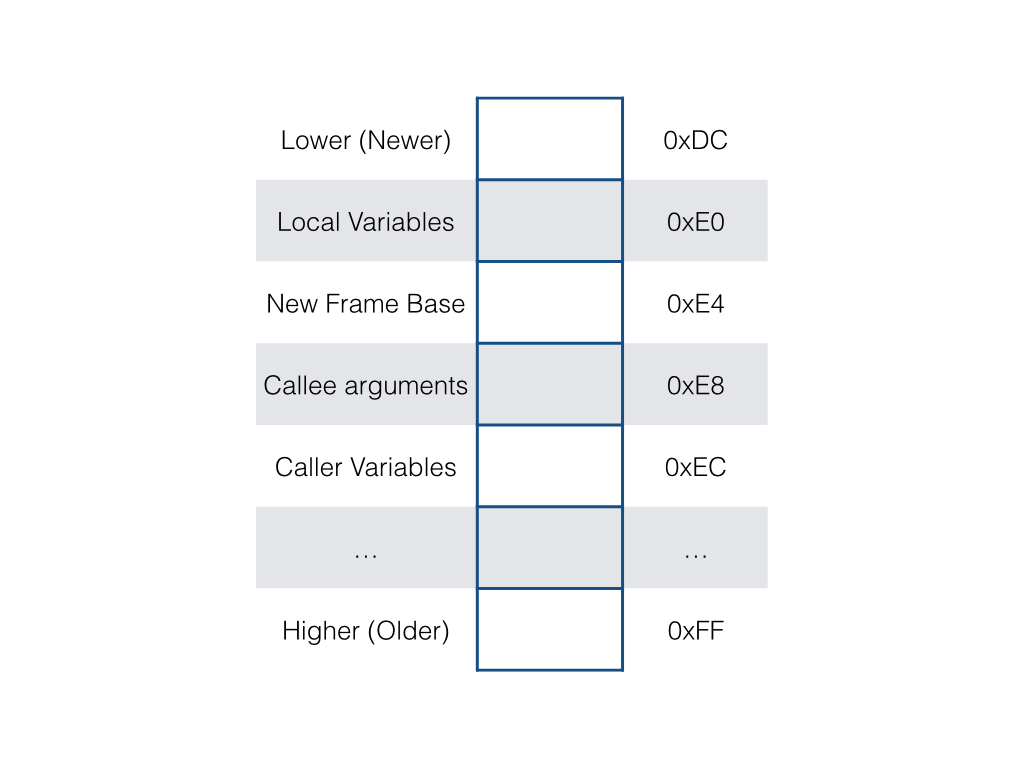
\includegraphics[width = 0.65\textwidth]{./images/stack.jpg} \caption{An example stack,
showing the dangerous arrangement of a function's arguments and its caller's local variables} \label{fig_stack}
\end{figure}

Format string functions are useful and powerful, but can be dangerous; Their intended use is along the line of {\tt
printf("\%x", x)} which prints the value of the variable {\tt x} interpreted as a hexadecimal integer. However, {\tt
printf} blindly trusts the format string to reflect the arguments. {\tt printf("\%x \%x \%x")} will print outthe values
of whatever is stored at the memory locations where the $2^{nd}$, $3^{rd}$ and $4^{th}$ arguments to printf should be if
they existed, without checking whether they exist or not. This means just using format specifiers we can start reading
memory from the stack that doesn't belong in the current context. If, then, we call {\tt printf("\%s\%s...\%s")}, the
program will tear values from the stack, interpret them as memory addresses that contain null-terminated strings, and
attempt to deference and print them. This will segfault quickly as the program attempts to access unauthorised
addresses. Similarly {\tt printf("\%n\%n...\%n")} will tear addresses from the stack, dereference them, set those
locations to 0x0, and again crash when it hits an invalid address.

With the version of the program that requested an integer input, both our attacks used that input as the target address.
In the subsequent version we both used the format string itself to determine where to write. In the first case, we
simply supply the appropriate address in integer form, converted from the output printed by the program. This location
is equivalent (when stack protectors are disabled) to where the 9th 4-byte argument to a printf call would sit. Thus
{\tt printf("\%8x\%8x\%8x\%8x\%8x\%8x\%8x\%8x\%n")} will dig eight words from the stack to the integer input by the
user, then set the value at that memory address to 64 = 0x40. Using another {\tt\%x} would read the data. You can also
leverage positional argument syntax to directly investigate the stack without changing it, which Drum chose to implement
in all of his attacks. Using that syntax, reading the ninth integer would look like this: {\tt printf("\%9\$8x")}, and
writing to it would be {\tt printf("\%9\$n")}.

Setting the address to large values like {\tt 0xd09f00d} can be very difficult, since this requires an exceptionally
long string.

Both of our memory alteration attacks use the {\tt \%n} format specifier to write to an arbitrary value to the memory
address of {\tt secret[1]}. For contrast we decided to use alternate methods of padding the format string to the correct
byte length.

Drum's attack used a padding specifier to an unsigned integer format specifier, or omitted the integer entirely, which
allows for the writing of values less than the printed length of the smallest stack variable. Writing a value of 0 to
{\tt secret[1]} without using this method and positional arguments is impossible. Tim's attack uses the more
tried-and-tested approach of standard stack popping, meaning that the minimum writeable value is determined by the
values in the stack and the width specifiers used when they are printed.

\subsection{Attack 2, riding the NOP Sled}

The exploit we used is based on the standard NOP sled and stack smashing approach, where we clobber the stack in order
to manipulate the return address of the current function. If the return pointer can be rewritten to point to the start
of the bytecode provided in the lab, then the running program will execute the bytecode and turn itself into a shell.
Unsafe string functions such as {\tt strcpy} will write strings past the end of their buffer, if not terminated,
regardless of how wide the buffer actually is. By writing a sufficiently long string, we can overflow the buffer and
overwrite memory lower down (higher memory addresses) on the stack, such as the return pointer.

Precisely engineering the return pointer to point exactly to the shellcode's location is often difficult. Though this
would be possible in this example without memory randomization, where we have GDB and access to the source code, when
memory address randomization is enabled it still becomes very difficult. A NOP sled gives us a larger target.
We construct our sled generally as follows:

An address which is somewhere earlier in the stack than the start of the current frame's return pointer is repeated
(endian-ness accounted for, avoiding null bytes) several times until it would clobber the return address. Then a large
series of no-operation instructions in precompiled bytecode is prepended to the shellcode, and this new blob is appended
to the repeated addresses. Jumping the execution into any one of those NOPs will cause the program to slide down its own
stack directly into the shellcode payload, making memory addresses much easier to guess.

In order to ensure that the resulting shell is indeed a root shell, we need to invoke a {\tt setuid} before launching a
shell. There are a few ways to make this modification to the shellcode -- Tim chose to copy the assembly code from the
assignment sheet, and add some extra lines to make this call. {\tt xorl \%ebx \%ebx} will set the general-purpose
register {\tt \%ebx} to 0. {\tt lea 0x17(\%ebx) \%eax} is designed for computing memory addresses, but here we use it to
add {\tt 0x17} to {\tt \%ebx} and store the result in {\tt \%eax}. {\tt int \$0x80} triggers interrupt {\tt 0x80}, a
syscall interrupt. Syscalls are parametrised exclusively by registers\cite{syscalls}. The first parameter is {\tt \%eax
= 0x17}, and tells the kernel to execute {\tt syscall[0x17]}, namely {\tt setuid}. The second is {\tt \%ebx = 0x0},
which is passed as a parameter into {\tt setuid}. {\tt setuid(0)} sets the user id to 0, more commonly known as {\tt
root}. When this call is placed before the code to launch a shell, the shell will be launched with root privileges.
Assembling this and skimming over the bytecode, we find that prepending the payload with {\tt 0x31db8d4317cd80} will get
the job done. Drum simply chose to delegate all shellcode generation to the metasploit framework, replacing the given
shellcode entirely.
